% ----------------------------------------------------------
% Apêndices
% Documentos gerados pelo próprio autor
% ----------------------------------------------------------

% ---
% Inicia os apêndices
% ---
\begin{apendicesenv}
	
	% Imprime uma página indicando o início dos apêndices
	\partapendices
	
	\chapter{Especificações de Casos de Uso}
	\label{casos-de-uso-especificacao}
	
	
	\begin{itemize}
		\item UC01: Fazer Login - Este uso de caso é abordado quando o cliente for fazer um cadastro na plataforma. O \autoref{casos-de-uso1} informa uma descrição, o fluxo básico de cadastro, um fluxo alternativo, pré-condições necessárias para conseguir fazer o uso de caso e pós-condições quando o uso de caso é concluído com sucesso.\\			
	\end{itemize}

\begin{quadro}[htb]
	\centering
	\ABNTEXfontereduzida
	\caption[Caso de Uso Fazer Login]{Caso de Uso Fazer Login}
	\label{casos-de-uso1}
\end{quadro}
\begin{longtable}{|p{3.3cm}|p{12.3cm}|}
	\hline
	\thead{} & \thead{Ator} \\
	\hline
	\endfirsthead
	%
	\multicolumn{2}{c}{\scriptsize Fonte: Equipe diversaGente (2022).}%
	{{\bfseries \autoref{casos-de-uso1} continued from previous page}} \\
	\endhead
	Descrição & Ao realizar o processo de login, o usuário terá acesso a todas as funcionalidades do aplicativo como consultar o feed de notícias, ter acesso ao fórum podendo criar subcategorias e post e compartilhar informações nos canais de texto, enviar mensagens privadas a outras pessoas que também estão logadas no app e avaliar locais a partir da sua vivência deste estabelecimento \\
	\hline
	Fluxo Básico  & 
	\begin{enumerate}
		\item O usuário entra no aplicativo e visualiza a tela de login;
		\item O usuário insere seu email e senha;
		\item Usuário entra no aplicativo;
		\item O caso de uso é encerrado. 
	\end{enumerate}\\
	\hline
	Fluxo Alternativo  & O usuário esqueceu a senha:
	\begin{enumerate}
		\item O usuário entra no aplicativo e visualiza a tela de login;
		\item O usuário insere seu email e senha;
		\item O sistema informa que a senha inserida está incorreta.
		\item O usuário clica em "Esqueci minha senha";
		\item O sistema envia um e-mail para o ator para trocar a senha;
		\item O usuário abre o e-mail e redefine sua senha;
		\item O fluxo principal é recomeçado.
		\item O caso de uso é encerrado.
	\end{enumerate} \\
	\hline
	Fluxo Alternativo  &  Preenchimento incorreto da senha:
	\begin{enumerate}
		\item O usuário entra no aplicativo e visualiza a tela de login;
		\item O usuário insere seu email e senha;
		\item O sistema informa que a senha inserida está incorreta.
		\item O sistema informa que a senha inserida está incorreta.
		\item O caso de uso é encerrado. 
	\end{enumerate}\\
	\hline
	Fluxo Alternativo & Primeiro Acesso
	\begin{enumerate}
		\item O usuário entra no aplicativo e visualiza a tela de login;
		\item O usuário clica em "cadastrar";
		\item O sistema apresenta a tela de boas vindas;
		\item O usuário clica em "Avançar"
		\item O usuário insere as informações necessárias para o cadastramento no aplicativo;
		\item O usuário recebe a mensagem de "Cadastro feito com sucesso";
		\item O fluxo principal é começado para o usuário;
		\item O caso de uso é encerrado.
	\end{enumerate} \\
	\hline
	Fluxo Alternativo & Login Social (Google):
	\begin{enumerate}
		\item O usuário entra no aplicativo e visualiza a tela de login;
		\item O usuário clica no botão de realizar o login social;
		\item O sistema direciona o usuário para link do login social;
		\item O usuário faz sua autenticação com o email social e senha;
		\item O usuário retorna para tela do aplicativo já sendo direcionado para o fluxo principal do app;
		\item O caso de uso é encerrado. 
	\end{enumerate} \\
	\hline
	Pré-condições & Ter acesso à internet, o aplicativo previamente instalado e uma conta Google.
	\hline
	Pós-condições & Acesso a homepage do aplicativo e de todas as funcionalidades existentes no sistema. \\
	\hline
\end{longtable}
\fonte{Equipe diversaGente (2022)}


%--------------------------------------------------------------

\begin{itemize}
	\item UC02: Efetuar Cadastro - Este uso de caso é abordado quando o cliente for fazer um cadastro na plataforma. O 	\autoref{casos-de-uso2} informa uma descrição, o fluxo básico de cadastro, um fluxo alternativo, pré-condições necessárias para conseguir fazer o uso de caso e pós-condições quando o uso de caso é concluído com sucesso. \\
\end{itemize}


\begin{quadro}[htb]
	\centering
	\ABNTEXfontereduzida
	\caption[Caso de Uso Efetuar Cadastro]{Caso de Uso Efetuar Cadastro}
	\label{casos-de-uso2}
\end{quadro}
\begin{longtable}{|p{3.3cm}|p{12.3cm}|}
	\hline
	\thead{} & \thead{Ator} \\
	\hline
		\endfirsthead
	%
	\multicolumn{2}{c}{\scriptsize Fonte: Equipe diversaGente (2022).}%
	{{ \autoref{casos-de-uso2} continued from previous page}} \\
	\endhead
	Descrição & Esse caso terá como funcionalidade o cadastrar novos usuários na aplicação.\\
	\hline
	Fluxo Básico  & 
	\begin{enumerate}
		\item O usuário entra no aplicativo e visualiza a tela de login;
		\item O usuário clica em "cadastrar";
		\item O sistema apresenta a tela de boas vindas;
		\item O usuário clica em "Avançar";
		\item O usuário clica em "Cadastrar no App";
		\item O usuário insere as informações necessárias para o cadastramento no aplicativo;
		\item É retornado ao usuário: "Cadastro realizado com sucesso";
		\item O fluxo principal é começado para o usuário;
		\item O caso de uso é encerrado.. 
	\end{enumerate}\\
	\hline
	Fluxo Alternativo  & Cadastro com a conta Google:
	\begin{enumerate}
		\item O usuário entra no aplicativo e visualiza a tela de login;
		\item O usuário clica em "cadastrar";
		\item O sistema apresenta a tela de boas vindas;
		\item O usuário clica em "Avançar";
		\item O usuário clica em "Cadastrar com o Google";
		\item O sistema irá direcioná-lo para sua conta google para permitir acesso;
		\item O usuário é retornado para o aplicativo e recebe a mensagem de "Cadastro feito com sucesso";
		\item  O fluxo principal é começado para o usuário;
		\item O caso de uso é encerrado.
	\end{enumerate}\\
	\hline
	Pré-condições & Ter acesso à internet e o aplicativo previamente instalado.\\
	\hline
	Pós-condições & O Visitante vai se tornar um novo usuário da aplicação.\\
	\hline
\end{longtable}
\fonte{Equipe diversaGente (2022)}


%--------------------------------------------------------------
	
	\begin{itemize}
		\item UC03: Editar perfil -  Este uso de caso é abordado quando o cliente for editar o seu perfil na plataforma.
		O \autoref{casos-de-uso3} informa uma descrição, o fluxo básico de cadastro, um fluxo alternativo, pré-
		condições necessárias para conseguir fazer o uso de caso e pós-condições quando o uso de
		caso é concluído com sucesso. \\
		
	\end{itemize}
	
	
	\begin{quadro}[htb]
		\centering
		\ABNTEXfontereduzida
		\caption[Caso de Uso Editar Perfil]{Caso de Uso Editar Perfil}
		\label{casos-de-uso3}
	\end{quadro}	
	\begin{longtable}{|p{3.3cm}|p{12.3cm}|}
		\hline
		\thead{} & \thead{Ator} \\
		\hline
		
		\endfirsthead
		%
		\multicolumn{2}{c}{\scriptsize Fonte: Equipe diversaGente (2022).}%
		{{ \autoref{casos-de-uso3} continued from previous page}} \\
		\endhead
		
		Descrição & Esse caso de uso ocorre quando o usuário logado no aplicativo deseja alterar suas informações de perfil.\\
		\hline
		Fluxo Básico  &
		\begin{enumerate}
			\item O usuário seleciona a seção "Perfil";
			\item O usuário seleciona "Editar Perfil";
			\item O sistema exibe os dados do perfil: nome, data de nascimento, e-mail, neuro diversidades que tem interesse, abertura de mensagens privadas;
			\item O usuário seleciona o(s) dado(s) que deseja editar;
			\item O usuário atualiza as suas informações e pressiona no botão "Salvar";
			\item O sistema valida os dados conforme requeridos e atualiza o perfil do assinante;
			\item O caso de uso é encerrado. 
		\end{enumerate}\\
		\hline
		Pré-condições & Ter acesso à internet e estar previamente logado no aplicativo.\\
		\hline
		Pós-condições & Ao final das alterações feitas pelo usuário, a seção perfil deve estar atualizada.\\
		\hline
	\end{longtable}
	\fonte{Equipe diversaGente (2022)}
	
	%--------------------------------------------------------------
	
	\begin{itemize}
		\item UC04: Consultar mensagens no Fórum - Este uso de caso é abordado quando o cliente for editar o seu perfil na plataforma.
		O \autoref{casos-de-uso4} informa uma descrição, o fluxo básico de cadastro, um fluxo alternativo, pré-
		condições necessárias para conseguir fazer o uso de caso e pós-condições quando o uso de
		caso é concluído com sucesso. \\
		
	\end{itemize}
	
	\begin{quadro}[htb]
		\centering
		\ABNTEXfontereduzida
		\caption[Caso de Uso Consultar mensagens do Fórum]{Caso de Uso Consultar mensagens do Fórum}
		\label{casos-de-uso4}
	\end{quadro}
	\begin{longtable}{|p{3.3cm}|p{12.3cm}|}
		\hline
		\thead{} & \thead{Ator} \\
		\hline
				
		\endfirsthead
		%
		\multicolumn{2}{c}{\scriptsize Fonte: Equipe diversaGente (2022).}%
		{{ \autoref{casos-de-uso4} continued from previous page}} \\
		\endhead
		
		Descrição & O cliente deve encontrar todas as mensagens ocorridas dentro das subcategorias.\\
		\hline
		Fluxo Básico  & 
		\begin{enumerate}
			\item O usuário seleciona a seção "Fórum";
			\item O usuário seleciona a categoria desejada;
			\item O sistema mostra todas as subcategorias relacionadas categoria escolhida pelo usuário;
			\item O usuário escolhe uma subcategoria;
			\item O sistema mostra todas as mensagens ocorridas nesse canal de texto até o momento. 
			\item O caso de uso é encerrado.
		\end{enumerate}\\
		\hline
		Pré-condições & Ter acesso à internet e estar previamente logado no aplicativo.\\
		\hline
		Pós-condições & Ao final da escolha da subcategoria, deverá mostrar todas as mensagens do canal de texto.\\
		\hline
	\end{longtable}
	\fonte{Equipe diversaGente (2022)}
	
%--------------------------------------------------------------
	
	\begin{itemize}
		\item UC05: Remover mensagens no Fórum -Este uso de caso é abordado quando o cliente remover mensagens no fórum. O 	\autoref{casos-de-uso5} informa uma descrição, o fluxo básico de cadastro, pré-condições necessárias para conseguir fazer o uso de caso e pós-condições quando o uso de caso é concluído com sucesso. \\
	\end{itemize}

	
	\begin{quadro}[htb]
		\centering
		\ABNTEXfontereduzida
		\caption[Caso de Uso Remover mensagens no Fórum]{Caso de Uso Remover mensagens no Fórum}
		\label{casos-de-uso5}
	\end{quadro}
	\begin{longtable}{|p{3.3cm}|p{12.3cm}|}
		\hline
		\thead{} & \thead{Ator} \\
		\hline
						
		\endfirsthead
		%
		\multicolumn{2}{c}{\scriptsize Fonte: Equipe diversaGente (2022).}%
		{{ \autoref{casos-de-uso5} continued from previous page}} \\
		\endhead
		
		Descrição & Ao criar uma subcategoria, o cliente poderá excluir sua própria mensagem dentro do canal de texto e poderá excluir as mensagens de outros dentro dessa subcategoria que ele criou. O Administrador terá permissão de excluir as mensagens das subcategorias, até mesmo do criador dela.\\
		\hline
		Fluxo Básico  & 
		Para o cliente:
		\begin{enumerate}
			\item O usuário seleciona a seção "Fórum";
			\item O usuário seleciona a categoria desejada;
			\item O sistema mostra todas as subcategorias relacionadas à categoria escolhida pelo usuário;
			\item O usuário escolhe uma subcategoria;
			\item O sistema mostra todas as mensagens ocorridas nesse canal de texto até o momento. 
			\item O usuário seleciona a mensagem que deseja excluir;
			\item O sistema atualiza o canal de texto retirando a mensagem excluída. 
			\item O  caso de uso é encerrado. 
		\end{enumerate}\\
		\hline
		Fluxo Básico  & 
		Para o Administrador:
		\begin{enumerate}
			\item O administrador seleciona a seção "Fórum";
			\item O administrador seleciona a categoria desejada;
			\item O administrador mostra todas as subcategorias relacionadas à categoria escolhida pelo usuário;
			\item O administrador escolhe uma subcategoria;
			\item O sistema mostra todas as mensagens ocorridas nesse canal de texto até o momento. 
			\item O administrador seleciona a mensagem que deseja excluir;
			\item O sistema atualiza o canal de texto retirando a mensagem excluída. 
			\item O caso de uso é encerrado. 
		\end{enumerate}\\
		\hline
		Pré-condições & Para o Cliente: 
		
		O cliente deve estar logado no app e ser o criador do subcategoria escolhida.\\
		\hline
		Pré-Condições & Para o Administrador:
		
		Deve-ser ter o permissionamento de acesso necessário.
		\hline
		Pós-condições & O sistema deve atualizar o canal de texto já retirando a mensagem de texto excluída.
		\hline
	\end{longtable}
	\fonte{Equipe diversaGente (2022)}
	
%--------------------------------------------------------------
	
	\begin{itemize}
		\item UC06: Curtir mensagens no Fórum. Este uso de caso é abordado quando o cliente for curtir uma mensagem do fórum. O 	\autoref{casos-de-uso6} informa uma descrição, fluxo básico, pré-condições e  pós-condições.\\
	\end{itemize}

	\begin{quadro}[htb]
		\centering
		\ABNTEXfontereduzida
		\caption[Caso de Uso Curtir mensagens no Fórum]{Caso de Uso Curtir mensagens no Fórum}
		\label{casos-de-uso6}
	\end{quadro}

\pagebreak

		\begin{longtable}{|p{3.3cm}|p{12.3cm}|}
		\hline
		\thead{} & \thead{Ator} \\
		\hline
		Descrição & O usuário poderá curtir uma mensagem de texto dentro das subcategorias.\\
		\hline
						
		\endfirsthead
		%
		\multicolumn{2}{c}{\scriptsize Fonte: Equipe diversaGente (2022).}%
		{{ \autoref{casos-de-uso6} continued from previous page}} \\
		\endhead
		
		Fluxo Básico  & 
		\begin{enumerate}
			\item O usuário seleciona a seção "Fórum";
			\item O usuário seleciona a categoria desejada;
			\item O sistema mostra todas as subcategorias relacionadas categoria escolhida pelo usuário;
			\item O usuário escolhe uma subcategoria;
			\item O sistema mostra todas as mensagens ocorridas nesse canal de texto até o momento. 
			\item  O usuário seleciona a mensagem desejada e clica em "curtir mensagem";
			\item  O sistema atualiza o canal de texto;
			\item  O caso de uso é encerrado;
		\end{enumerate}\\
		\hline
		Pré-condições & Ter acesso à internet e estar previamente logado no aplicativo.\\
		\hline
		Pós-condições & O sistema irá atualizar o número de curtidas da mensagem selecionada pelo usuário.\\
		\hline
	
	\end{longtable}
	\fonte{Equipe diversaGente (2022)}
	
	\pagebreak

%--------------------------------------------------------------
	
	\begin{itemize}
		\item UC07: Criar categoria - Este uso de caso é abordado quando o cliente for curtir uma mensagem do fórum. O 	\autoref{casos-de-uso7}	informa uma descrição, o fluxo básico de cadastro, pré-condições necessárias para conseguir fazer o uso de caso e pós-condições quando o uso de caso é concluído com sucesso.\\
	\end{itemize}
	
	\begin{quadro}[htb]
		\centering
		\ABNTEXfontereduzida
		\caption[Caso de Uso Criar categoria]{Caso de Uso Criar categoria}
		\label{casos-de-uso7}
	\end{quadro}

	\begin{longtable}{|p{3.3cm}|p{12.3cm}|}
		\hline
		\thead{} & \thead{Ator} \\
		\hline
								
		\endfirsthead
		%
		\multicolumn{2}{c}{\scriptsize Fonte: Equipe diversaGente (2022).}%
		{{ \autoref{casos-de-uso7} continued from previous page}} \\
		\endhead
		
		Descrição & O Administrador tem permissão de criar uma categoria dentro do fórum.\\
		\hline
		Fluxo Básico  & 
		\begin{enumerate}
			\item O administrador seleciona a seção "Fórum";
			\item O administrador seleciona o botão "+";
			\item O sistema irá apresentar a opção "Criar uma Categoria";
			\item Ao clicar em criar uma categoria, o administrador deverá escrever o nome da categoria e clicar em "Criar canal de texto";
			\item O sistema atualizará com a nova categoria criada. 
			\item O caso de uso é encerrado. 
		\end{enumerate}\\
		\hline
		Pré-condições &O administrador deve ter a chave de permissão.
		\hline
		Pós-condições & O sistema mostrará a nova categoria criada pelo administrador e deve permitir que a partir dessa categoria sejam criadas subcategorias pelos usuários e administradores.\\
		\hline
	\end{longtable}
	\fonte{Equipe diversaGente (2022)}
		
%--------------------------------------------------------------
	
	\begin{itemize}
		\item UC08: Criar uma subcategoria - Este uso de caso é abordado quando o cliente for criar uma subcategoria. O \autoref{casos-de-uso8}	informa uma descrição, o fluxo básico de cadastro, pré-condições necessárias para conseguir fazer o uso de caso e pós-condições quando o uso de caso é concluído com sucesso.\\
	\end{itemize}

\pagebreak
	
	\begin{quadro}[htb]
		\centering
		\ABNTEXfontereduzida
		\caption[Caso de Uso Criar uma subcategoria]{Caso de Uso Criar uma subcategoria}
		\label{casos-de-uso8}
	\end{quadro}
	\begin{longtable}{|p{3.3cm}|p{12.3cm}|}
		\hline
		\thead{} & \thead{Ator} \\
		\hline
									
		\endfirsthead
		%
		\multicolumn{2}{c}{\scriptsize Fonte: Equipe diversaGente (2022).}%
		{{ \autoref{casos-de-uso8} continued from previous page}} \\
		\endhead
		
		Descrição & O cliente e/ou administrador devem conseguir criar subcategorias a partir das categorias já criadas pelo administrador.\\
		\hline
		Fluxo Básico  & 
		\begin{enumerate}
			\item O usuário seleciona a seção "Fórum";
			\item O usuário seleciona a categoria desejada;
			\item O usuário clica no botão "+" ao lado do nome da categoria selecionada;
			\item O usuário escreve o nome da subcategoria e clica em "Salvar"
			\item O sistema atualiza com a nova subcategoria criada. 
			\item O caso de uso é encerrado. 
		\end{enumerate}
		\hline
		Pré-condições & O cliente deve estar logado no app e o administrador deve ter a chave de permissão;
		\hline
		Pós-condições & O sistema mostrará a nova categoria criada pelo administrador ou usuário.\\
		\hline
	\end{longtable}
	\fonte{Equipe diversaGente (2022)}
	
%---------------------------------------------------------------
	
	\begin{itemize}
		\item UC09: Remover uma subcategoria - Este uso de caso é abordado quando o cliente for remover uma subcategoria. O 	\autoref{casos-de-uso9}	informa uma descrição, o fluxo básico de cadastro, pré-condições necessárias para conseguir fazer o uso de caso e pós-condições quando o uso de caso é concluído com sucesso.\\
	\end{itemize}
	
	\begin{quadro}[htb]
		\centering
		\ABNTEXfontereduzida
		\caption[Caso de Uso Remover uma subcategoria]{Caso de Uso Remover uma subcategoria}
		\label{casos-de-uso9}
	\end{quadro}
	
	\begin{longtable}{|p{3.3cm}|p{12.3cm}|}
		\hline
		\thead{} & \thead{Ator} \\
		\hline
							
		\endfirsthead
		%
		\multicolumn{2}{c}{\scriptsize Fonte: Equipe diversaGente (2022).}%
		{{ \autoref{casos-de-uso9} continued from previous page}} \\
		\endhead
		Descrição & O cliente e/ou administrador devem conseguir remover uma subcategoria. \\
		\hline
		Fluxo Básico  & Para o cliente
		\begin{enumerate}
			\item O usuário seleciona a seção "Fórum";
			\item O usuário seleciona uma categoria;
			\item O sistema mostra todas as subcategoria existentes;
			\item O cliente seleciona a subcategoria desejada;
			\item O cliente pressiona a subcategoria;
			\item Caso o cliente seja o criador dessa subcategoria, o sistema irá mostrar uma pop-up perguntando para o usuário se ele deseja excluir a subcategoria criada. 
			\item O usuário clica em "Sim";
			\item O sistema exclui a subcategoria;
			\item O caso de uso é encerrado. 
		\end{enumerate}
		\hline
		Fluxo Básico  & Para o administrador
		\begin{enumerate}
			\item O administrador seleciona a seção "Fórum";
			\item O administrador seleciona uma categoria;
			\item O sistema mostra todas as subcategoria existentes;
			\item O administrador seleciona a subcategoria desejada;
			\item O administrador pressiona a subcategoria;
			\item O sistema irá mostrar uma pop-up perguntando para o administrador se ele deseja excluir a subcategoria pressionada;
			\item O administrador clica em "Sim";
			\item O sistema exclui a subcategoria;
			\item O caso de uso é encerrado. 
		\end{enumerate}\\
		\hline
		Pré-condições & Para o cliente:
		
		O cliente deve estar logado no app e ser o criador do subcategoria escolhida. \\
		\hline
		Pré-condições & Para o administrador:
		
		Deve-ser ter o permissionamento de acesso necessário.
		\hline
		Pós-condições & O sistema irá atualizar removendo a subcategoria selecionada.\\
		\hline
	\end{longtable}
	\fonte{Equipe diversaGente (2022)}
	
	%-----------------------------------------------------------
	
	\begin{itemize}
		\item UC10: Criação do Local Avaliado - Este uso de caso é abordado quando o cliente for criar um local para ser avaliado. O \autoref{casos-de-uso10} informa uma descrição, o fluxo básico de cadastro, um fluxo de exceção, pré-condições necessárias para conseguir fazer o uso de caso e pós-condições quando o uso de caso é concluído com sucesso.\\	
	\end{itemize}
		
	\begin{quadro}[htb]
		\centering
		\ABNTEXfontereduzida
		\caption[Caso de Uso Criação do Local Avaliado]{Caso de Uso Criação do Local Avaliado}
		\label{casos-de-uso10}
	\end{quadro}
	\begin{longtable}{|p{3.3cm}|p{12.3cm}|}
		\hline
		\thead{} & \thead{Ator} \\
		\hline
		
										
		\endfirsthead
		%
		\multicolumn{2}{c}{\scriptsize Fonte: Equipe diversaGente (2022).}%
		{{ \autoref{casos-de-uso10} continued from previous page}} \\
		\endhead
		
		Descrição & O usuário poderá avaliar positivamente ou negativamente os estabelecimentos que ele queira recomendar para outras pessoas dentro da rede social.\\
		\hline
		Fluxo Básico  & 
		\begin{enumerate}
			\item O usuário clica na seção 'Locais Avaliados';
			\item O usuário clica na aba 'Meus Locais Avaliados';
			\item O usuário clica em "Adicionar Avaliação";
			\item O sistema fornece a parte de "Adicionar Avaliação";
			\item O usuário cadastra a avaliação e clica em "Salvar";
			\item O sistema busca identificar e confirmar os dados inseridos pelo usuário.
			\item O sistema retorna "Avaliação Adicionada" e adiciona na lista de locais avaliados;
			\item O caso de uso é encerrado.
		\end{enumerate}
		\hline
		Fluxo de Exceção & O usuário não insere todos os dados necessários: 
		\begin{enumerate}
			\item O usuário clica na aba 'Meus Locais Avaliados';
			\item O usuário clica em "Adicionar Avaliação";
			\item O sistema fornece a parte de "Adicionar Avaliação";
			\item O usuário cadastra a avaliação e clica em "Salvar";
			\item O sistema retorna os dados obrigatórios que o usuário não inseriu ao cadastrar e impede que a avaliação seja salva;
			\item O caso de uso é encerrado. 
		\end{enumerate}
		\hline
		Pré-condições & Ter acesso à internet e estar previamente logado no aplicativo.
		\hline
		Pós-condições & Apresentar o Local Avaliado cadastrado pelo usuário na aba ’Locais Avaliados’.
		\hline
	\end{longtable}
	\fonte{Equipe diversaGente (2022)}
	\pagebreak
	
%---------------------------------------------------------------
	
	\begin{itemize}
		\item UC11: Consultar Locais Avaliados - Este uso de caso é abordado quando o cliente for consultar locais avaliados. O \autoref{casos-de-uso11} informa uma descrição, o fluxo básico de cadastro, pré-condições necessárias para conseguir fazer o uso de caso e pós-condições quando o uso de caso é concluído com sucesso.	
	\end{itemize}
	
	\begin{quadro}[htb]
		\centering
		\ABNTEXfontereduzida
		\caption[Caso de Uso Consultar Locais Avaliados]{Consultar Locais Avaliados}
		\label{casos-de-uso11}
	\end{quadro}
	\begin{longtable}{|p{3.3cm}|p{12.3cm}|}
		\hline
		\thead{} & \thead{Ator} \\
		\hline
										
		\endfirsthead
		%
		\multicolumn{2}{c}{\scriptsize Fonte: Equipe diversaGente (2022).}%
		{{ \autoref{casos-de-uso11} continued from previous page}} \\
		\endhead
		
		Descrição & Consultar todos os locais avaliados já adicionados pelos usuários.\\
		\hline
		Fluxo Básico  & 
		\begin{enumerate}
			\item O usuário clica na seção 'Locais Avaliados';
			\item O usuário clica na aba 'Todos Locais Avaliados';  
			\item O usuário clica no nome de um local avaliado;
			\item O usuário visualiza a avaliação;
			\item O caso de uso é encerrado. 
		\end{enumerate}\\
		\hline
		Pré-condições & Ter acesso à internet e estar previamente logado no aplicativo.
		\hline
		Pós-condições & Apresentar todos os locais avaliados cadastrados e seus respectivos dados.\\
		\hline
	\end{longtable}
	\fonte{Equipe diversaGente (2022)}
	
	%---------------------------------------------------------------
	
	\begin{itemize}
		\item UC12: Editar Locais Avaliados - Este uso de caso é abordado quando o cliente for editar um local avaliado. O 	\autoref{casos-de-uso12} informa uma descrição, o fluxo básico de cadastro, pré-condições necessárias para conseguir fazer o uso de caso e pós-condições quando o uso de caso é concluído com sucesso.\\
	\end{itemize}
		
	\begin{quadro}[htb]
		\centering
		\ABNTEXfontereduzida
		\caption[Caso de Uso Editar Locais Avaliados]{Caso de Uso Editar Locais Avaliados}
		\label{casos-de-uso12}
	\end{quadro}
	\begin{longtable}{|p{3.3cm}|p{12.3cm}|}
		\hline
		\thead{} & \thead{Ator} \\
		\hline
		
										
		\endfirsthead
		%
		\multicolumn{2}{c}{\scriptsize Fonte: Equipe diversaGente (2022).}%
		{{ \autoref{casos-de-uso12} continued from previous page}} \\
		\endhead
		
		Descrição & O usuário poderá editar as informações inseridas por ele na aba de 'Meus Locais Avaliados'.\\
		\hline
		Fluxo Básico  &
		\begin{enumerate}
			\item O usuário clica na aba 'Meus Locais Avaliados';
			\item O usuário pressiona o local avaliado na qual ele quer editar;
			\item O sistema mostra uma pop-up com a opção "Editar Local Avaliado";
			\item O usuário clica em "Editar Local Avaliado";
			\item O usuário edita as informações e clica em "Salvar";
			\item O sistema confirmar os dados inseridos pelo usuário;
			\item O caso de uso é encerrado. 
		\end{enumerate}
		\hline
		Pré-condições & Ter acesso à internet, estar logado no aplicativo e ser o criador do local avaliado em questão.
		\hline
		Pós-condições & O sistema deve apresentar o local avaliado com as novas informações inseridas pelo usuário.
		\hline
	\end{longtable}
	\fonte{Equipe diversaGente (2022)}
	%---------------------------------------------------------------
	
	\begin{itemize}
		\item UC13: Remover Local Avaliado - Este uso de caso é abordado quando o cliente remover um local avaliado. O \autoref{casos-de-uso13} informa uma descrição, o fluxo básico de cadastro, pré-condições necessárias para conseguir fazer o uso de caso e pós-condições quando o uso de caso é concluído com sucesso.\\		
	\end{itemize}
	
	\begin{quadro}[htb]
		\centering
		\ABNTEXfontereduzida
		\caption[Caso de Uso Remover Local Avaliado]{Caso de Uso Remover Local Avaliado}
		\label{casos-de-uso13}
	\end{quadro}
	\begin{longtable}{|p{3.3cm}|p{12.3cm}|}
		\hline
		\thead{} & \thead{Ator} \\
		\hline
										
		\endfirsthead
		%
		\multicolumn{2}{c}{\scriptsize Fonte: Equipe diversaGente (2022).}%
		{{ \autoref{casos-de-uso13} continued from previous page}} \\
		\endhead
		
		Descrição &O usuário poderá excluir o local avaliado inserido por ele na aba de 'Meus Locais Avaliados'.\\
		\hline
		Fluxo Básico  & 
		\begin{enumerate}
			\item O usuário clica na seção 'Locais Avaliados';
			\item O usuário clica na aba 'Meus Locais Avaliados';
			\item O usuário pressiona o local avaliado na qual ele quer excluir;
			\item O sistema mostra uma pop-up com a opção "Excluir Local Avaliado"; 
			\item O usuário clica em "Excluir Local Avaliado";
			\item O usuário exclui local avaliado";
			\item O sistema atualiza e retorna com a mensagem "local excluído com sucesso";
			\item O caso de uso é encerrado. 
		\end{enumerate}\\
		\hline
		Pré-condições & Ter acesso à internet, estar previamente logado no aplicativo e ser o criador da avaliação de local em questão.
		\hline
		Pós-condições & O sistema deve excluir o local avaliado escolhido pelo usuário da lista "Meus Locais Avaliados" e "Locais Avalaidos".\\
		\hline
	\end{longtable}
	\fonte{Equipe diversaGente (2022)}
	
	%---------------------------------------------------------------
	
	\begin{itemize}
		\item UC14: Visualizar Perfil dos usuários - Este uso de caso é abordado quando o cliente for visualizar um perfil de um outro usuário na plataforma. O \autoref{casos-de-uso14} informa uma descrição, o fluxo básico de cadastro, um fluxo alternativo, pré-condições necessárias para conseguir fazer o uso de caso e pós-condições quando o uso de caso é concluído com sucesso.\\	
	\end{itemize}
	
	\pagebreak
	
	\begin{quadro}[htb]
		\centering
		\ABNTEXfontereduzida
		\caption[Caso de Uso Visualizar Perfil dos usuários]{Caso de Uso Visualizar Perfil dos usuários}
		\label{casos-de-uso14}
	\end{quadro}
	\begin{longtable}{|p{3.3cm}|p{12.3cm}|}
		\hline
		\thead{} & \thead{Ator} \\
		\hline
										
		\endfirsthead
		%
		\multicolumn{2}{c}{\scriptsize Fonte: Equipe diversaGente (2022).}%
		{{ \autoref{casos-de-uso14} continued from previous page}} \\
		\endhead
		
		Descrição & Visualiza perfil do cliente quando clica na foto de perfil ou no nome do usuário.\\
		\hline
		Fluxo Básico  & 
		\begin{enumerate}
			\item O usuário clica na imagem do usuário;
			\item O usuário visualiza o perfil de outro usuário;
			\item O caso de uso está encerrado.
		\end{enumerate}\\
		\hline
		Fluxo Alternativo & 
		\begin{enumerate}
			\item O usuário clica no nome do usuário;
			\item O usuário visualiza o perfil de outro usuário;
			\item O caso de uso está encerrado.
		\end{enumerate}\\
		\hline
		Pré-condições & Ter acesso à internet e estar logado previamente no aplicativo.\\
		\hline
		Pós-condições & O sistema irá mostrar uma nova tela com todas as informações do usuário escolhido.\\
		\hline
	\end{longtable}
	\fonte{Equipe diversaGente (2022)}
	
	%---------------------------------------------------------------
	
	\begin{itemize}
		\item UC15: Troca de mensagens de texto em chat individual - Este uso de caso é abordado quando o cliente for trocar uma mensagem de texto com outro perfil. O \autoref{casos-de-uso15} informa uma descrição, o fluxo básico de ação, um fluxo alternativo, pré-condições necessárias para conseguir fazer o uso de caso e pós-condições quando o uso de caso é concluído com sucesso.\\
	\end{itemize}
	
	\begin{quadro}[htb]
		\centering
		\ABNTEXfontereduzida
		\caption[Caso de Uso Troca de mensagens de texto em chat individual]{Caso de Uso Troca de mensagens de texto em chat individual}
		\label{casos-de-uso15}
	\end{quadro}
	
	\begin{longtable}{|p{3.3cm}|p{12.3cm}|}
		\hline
		\thead{} & \thead{Ator} \\
		\hline
		
										
		\endfirsthead
		%
		\multicolumn{2}{c}{\scriptsize Fonte: Equipe diversaGente (2022).}%
		{{ \autoref{casos-de-uso15} continued from previous page}} \\
		\endhead
		
		Descrição &Nesse caso de uso, o usuário poderá enviar e receber mensagens por meio de um chat privado entre os usuários.\\
		\hline
		Fluxo Básico  & 
		\begin{enumerate}
			\item O usuário clica na aba "Chat";
			\item O usuário clica em um dos usuários que estão em sua lista;
			\item O usuário envia mensagem;
			\item O caso de uso é encerrado. 
		\end{enumerate}\\
		\hline
		Fluxo Alternativo & 
		Primeira vez do usuário enviando mensagem. 
		\begin{enumerate}
			\item O usuário clica na imagem ou no nome do outro usuário;
			\item O usuário visualiza o perfil desse usuário;
			\item O usuário clica em "Enviar Mensagem";
			\item O sistema abre o chat entre esses dois usuários;
			\item O usuário envia a mensagem;
			\item O caso de uso é encerrado 
		\end{enumerate}\\
		\hline
		Pré-condições & Ter acesso à internet e estar previamente logado no aplicativo\\
		\hline
		Pós-condições & O usuário deve ter sua mensagem entregue e recebida pelo outro usuário.\\
		\hline
	\end{longtable}
	\fonte{Equipe diversaGente (2022)}
	
	%---------------------------------------------------------------
	
	\begin{itemize}
		\item UC16: Visualizar notícias -Este uso de caso é abordado quando o cliente quiser visualizar uma notícia dentro da plataforma. O \autoref{casos-de-uso16} informa uma descrição, o fluxo básico de ação, pré-condições necessárias para a realização do caso e pós-condições da ação.\\
	\end{itemize}
	
	\begin{quadro}[htb]
		\centering
		\ABNTEXfontereduzida
		\caption[Caso de Uso Visualizar notícias]{Caso de Uso Visualizar notícias}
		\label{casos-de-uso16}
	\end{quadro}
	\begin{longtable}{|p{3.3cm}|p{12.3cm}|}
		\hline
		\thead{} & \thead{Ator} \\
		\hline
		
										
		\endfirsthead
		%
		\multicolumn{2}{c}{\scriptsize Fonte: Equipe diversaGente (2022).}%
		{{ \autoref{casos-de-uso16} continued from previous page}} \\
		\endhead
		
		Descrição & O usuário deverá visualizar todas as notícias dentro da seção "Feed de notícias".\\
		\hline
		Fluxo Básico  & 
		\begin{enumerate}
			\item O usuário logado entra na seção "Feed de notícias";
			\item O usuário visualiza as notícias;
			\item O caso de uso é encerrado. 
		\end{enumerate}\\
		\hline
		Fluxo Alternativo &
		\begin{enumerate}
			\item O usuário logado entra na seção "Feed de notícias";
			\item O usuário visualiza as notícias;
			\item O usuário clica em uma notícia;
			\item O sistema leva o usuário para uma nova tela com os detalhamentos da notícia clicada pelo usuário;
			\item O caso de uso é encerrado. 
		\end{enumerate}\\
		\hline
		Pré-condições & Ter acesso à internet e estar previamente logado no aplicativo.\\
		\hline
		Pós-condições & O sistema deve mostrar as notícias relacionadas ao tema de crianças neuro diversas.\\
		\hline
	\end{longtable}
	\fonte{Equipe diversaGente (2022)}
	
	%---------------------------------------------------------------
	
	\begin{itemize}
		\item UC17: Criar um Post -Este uso de caso é abordado quando o cliente quiser criar uma postagem na plataforma. O 	\autoref{casos-de-uso17} informa uma descrição, o fluxo básico de ação, pré-condições necessárias para a realização do caso e pós-condições da ação.\\
	\end{itemize}
	
	\begin{quadro}[htb]
		\centering
		\ABNTEXfontereduzida
		\caption[Caso de Uso Criar um Post]{Caso de Uso Criar um Post}
		\label{casos-de-uso17}
	\end{quadro}
	\begin{longtable}{|p{3.3cm}|p{12.3cm}|}
		\hline
		\thead{} & \thead{Ator} \\
		\hline
		
										
		\endfirsthead
		%
		\multicolumn{2}{c}{\scriptsize Fonte: Equipe diversaGente (2022).}%
		{{ \autoref{casos-de-uso17} continued from previous page}} \\
		\endhead
		
		Descrição & O usuário poderá criar um post a partir das subcategorias existentes. \\
		\hline
		Fluxo Básico  & 
		\begin{enumerate}
			\item O usuário seleciona uma subcategoria selecionada;
			\item O usuário clica no botão "+" ao lado do nome da subcategoria selecionada para criar o post;
			\item O usuário insere as informações necessárias para a criação do post;
			\item O usuário clica em "Criar Post"; 
			\item O caso de uso é encerrado. 
		\end{enumerate}\\
		\hline
		Pré-condições & Ter acesso à internet e estar previamente logado no aplicativo.\\
		\hline
		Pós-condições & O sistema deve permitir a criação do post feita pelo usuário.\\
		\hline
	\end{longtable}
	\fonte{Equipe diversaGente (2022)}
	%---------------------------------------------------------------

	\begin{itemize}
		\item UC18: Remover um Post - Este uso de caso é abordado quando o cliente vai fazer a remoção de uma postagem previamente feita. O \autoref{casos-de-uso18} informa uma descrição, o fluxo básico de ação, um fluxo alternativo, pré-condições necessárias para a realização do caso e pós-condições da ação.\\
	\end{itemize}
\pagebreak
	\begin{quadro}[htb]
		\centering
		\ABNTEXfontereduzida
		\caption[Caso de Uso Remover um Post]{Caso de Uso Remover um Post}
		\label{casos-de-uso18}
	\end{quadro}

	\begin{longtable}{|p{3.3cm}|p{12.3cm}|}
		\hline
		\thead{} & \thead{Ator} \\
		\hline
												
		\endfirsthead
		%
		\multicolumn{2}{c}{\scriptsize Fonte: Equipe diversaGente (2022).}%
		{{ \autoref{casos-de-uso18} continued from previous page}} \\
		\endhead
		
		Descrição &O usuário poderá remover um post a partir das subcategorias existentes.\\
		\hline
		Fluxo Básico  & 
		\begin{enumerate}
			\item O usuário seleciona um post;
			\item O usuário clica na opção "Apagar Post";
			\item O sistema apaga o post criado pelo usuário;
			\item O caso de uso é encerrado.
		\end{enumerate}\\
		\hline
		Fluxo Alternativo & 
		O administrador remove um post
		\begin{enumerate}
			\item O administrador seleciona um post;
			\item O administrador clica na opção "Apagar Post";
			\item O sistema apaga o post criado pelo administrador;
			\item O caso de uso é encerrado. 
		\end{enumerate}\\
		\hline
		Pré-condições & Ter acesso à internet, estar previamente logado no aplicativo e já ter uma postagem própria criada.
		\hline
		Pós-condições & O sistema deve atualizar com o post excluído pelo usuário. \\
		\hline
	\end{longtable}
	\fonte{Equipe diversaGente (2022)}
	
	%---------------------------------------------------------------
	
	\begin{itemize}
		\item UC19: Comentar Post - Este uso de caso é abordado quando o cliente fizer um comentário em uma postagem. O \autoref{casos-de-uso19} informa uma descrição, o fluxo básico de ação, pré-condições necessárias para a realização do caso e pós-condições da ação.\\
	\end{itemize}
	
\pagebreak
	
	\begin{quadro}[htb]
		\centering
		\ABNTEXfontereduzida
		\caption[Caso de Uso Comentar Post]{Caso de Uso Comentar Post}
		\label{casos-de-uso19}
	\end{quadro}
	\begin{longtable}{|p{3.3cm}|p{12.3cm}|}
		\hline
		\thead{} & \thead{Ator} \\
		\hline
														
		\endfirsthead
		%
		\multicolumn{2}{c}{\scriptsize Fonte: Equipe diversaGente (2022).}%
		{{ \autoref{casos-de-uso19} continued from previous page}} \\
		\endhead
		
		Descrição & O usuário poderá comentar um post a partir das subcategorias existentes. \\
		\hline
		Fluxo Básico  & 
		\begin{enumerate}
			\item O usuário seleciona um post;
			\item O usuário clica na opção "Comentar";
			\item O usuário adiciona um comentário no post seleciona;
			\item O caso de uso é encerrado. 
		\end{enumerate}
		\hline
		Pré-condições & Ter acesso à internet e estar previamente logado no aplicativo
		\hline
		Pós-condições & O sistema deve mostrar o comentário do usuário no post selecionado.
		\hline
	\end{longtable}
	\fonte{Equipe diversaGente (2022)}
	
	%---------------------------------------------------------------
	
	\begin{itemize}
		\item UC20: Curtir Post - Este uso de caso é abordado quando o cliente realiza a ação de curtir uma postagem. O \autoref{casos-de-uso20} informa uma descrição, o fluxo básico de ação, pré-condições necessárias e pós-condições da ação.\\
		
		
	\end{itemize}
	
	\begin{quadro}[htb]
		\centering
		\ABNTEXfontereduzida
		\caption[Caso de Uso Curtir Post]{Caso de Uso Curtir Post}
		\label{casos-de-uso20}
	\end{quadro}
	\begin{longtable}{|p{3.3cm}|p{12.3cm}|}
		\hline
		\thead{} & \thead{Ator} \\
		\hline
														
		\endfirsthead
		%
		\multicolumn{2}{c}{\scriptsize Fonte: Equipe diversaGente (2022).}%
		{{ \autoref{casos-de-uso20} continued from previous page}} \\
		\endhead
		
		Descrição & O usuário poderá curtir um post criado na subcategoria.\\
		\hline
		Fluxo Básico  & 
		\begin{enumerate}
			\item O usuário seleciona um post;
			\item O usuário clica em "Curtir";
			\item O caso de uso é encerrado.
		\end{enumerate}\\
		\hline
		Pré-condições & Ter acesso à internet e estar previamente logado no aplicativo
		\hline
		Pós-condições & O sistema deve atualizar as curtidas realizadas no post do usuário.\\
		\hline
	\end{longtable}
	\fonte{Equipe diversaGente (2022)}
	\pagebreak
	
	%---------------------------------------------------------------
	
	\begin{itemize}
		\item UC21: Comentar notícias - Este uso de caso é abordado quando o cliente vai fazer um comentário em uma notícia. O \autoref{casos-de-uso21} informa uma descrição, o fluxo básico do comentário, pré-condições necessárias para ser possível comentar e as condições pós o comentário ser realizado.\\
	\end{itemize}
	
	\begin{quadro}[htb]
		\centering
		\ABNTEXfontereduzida
		\caption[Caso de Uso Comentar notícias]{Caso de Uso Comentar notícias}
		\label{casos-de-uso21}
	\end{quadro}
	\begin{longtable}{|p{3.3cm}|p{12.3cm}|}
		\hline
		\thead{} & \thead{Ator} \\
		\hline
																
		\endfirsthead
		%
		\multicolumn{2}{c}{\scriptsize Fonte: Equipe diversaGente (2022).}%
		{{ \autoref{casos-de-uso21} continued from previous page}} \\
		\endhead
		
		Descrição & O usuário deve conseguir comentar uma notícias na seção "Feed de notícias". \\
		\hline
		Fluxo Básico  & 
		\begin{enumerate}
			\item O usuário logado entra na seção "Feed de notícias";
			\item O usuário visualiza as notícias;
			\item O usuário clica em uma notícia;
			\item O sistema leva o usuário para uma nova tela com os detalhamentos da notícia clicada pelo usuário;
			\item O usuário escreve seu comentário;
			\item O usuário clica em "Comentar";
			\item O caso de uso é encerrado. 
		\end{enumerate}
		\hline
		Pré-condições & Ter acesso à internet e estar previamente logado no aplicativo
		\hline
		Pós-condições & Após o usuário salvar seu comentário, o sistema deve apresentar o comentário realizado pelo usuário; 
		\hline
	\end{longtable}
	\fonte{Equipe diversaGente (2022)}
	
		
	% ----------------------------------------------------------
	\chapter{Proposta Inicial}
	% ----------------------------------------------------------
	
	Esse apêndice trás a proposta inicial apresentada pela equipe. 
	
	\section{Ideia}
	
	O nosso Projeto Integrador tem como ideia uma rede social para pais de crianças atípicas. No intuito de desenvolver um aplicativo, temos a visão de construir funcionalidades que tragam informações, trocas de experiências, desenvolvimento de um perfil de acordo com o interesse do usuário, recomendações de lugares oportunos para seus filhos e realização de notificações que passam a integrar mais os pais como a nossa aplicação. 
	
	Sendo assim, passando por cada funcionalidade podemos destacar cada elas como: 
	
	
	
	
	
	\section{Feed de notícias:}
	Essa função terá como propósito informar os pais a respeito de como lidar quando temos filhos atípicos, quais são as característica que diferencia seus filhos, os tipos de crianças e adolescentes que podemos encontrar, assim como textos publicados na internet de educadores e profissionais da saúde que são especializados no assunto, sendo constantemente atualizados. 
	
	\section{Fórum:}
	Essa funcionalidade tem como o principal objetivo a troca de experiência. Vamos construir salas de conversa de texto divididos por categorias como: Saúde, Educação, Alimentação e Lazer. A partir dessas categorias, o utilizador conseguirá criar subcategorias e assim poder compartilhar informações, dúvidas e debates a respeito do seu interesse.
	
	Os fórum também serão organizados de forma que os mais relevantes fiquem em destaques. Serve também para as postagens em destaques, podendo ser curtidas e fixadas em cada categoria. 
	
	\section{Perfil:}
	Nesse local, basicamente, o usuário irá poder compartilhar informações sobre si mesmo e os seus interesses e até mesmo compartilhar a sua história e experiências na descrição do seu perfil. Assim, será possível maior identificação de outros usuários com o perfil descrito, podendo ter mais interações e conhecimentos a respeito de cada um dentro da nossa rede social. 
	
	\section{Comunicação Instantânea: }
	Nessa parte, temos a ideia que o usuário possa enviar e receber mensagens. Assim, essa comunicação mais privada pode estabelecer que informações sejam compartilhadas e resolvidas com mais velocidades. 
	
	\section{Localização: }
	No intuito de manter uma maior interação entre os usuários e compartilhamento de informações, a possibilidade de compartilhar a localização dentro do aplicativo serve para encontrar pessoas que possam ter crianças que possuem o mesmo tipo de  necessidades especiais e que estão próximas uma das outras, além disso será permitido compartilhar também locais que recebam ou são projetadas para crianças e adolescentes portadoras de deficiência como forma de recomendações para outros pais. 
	
	\section{Notificações: }
	Nessa interação, o nosso aplicativo conseguirá fornecer mensagens que exibirá fora da UI do app para fornecer comunicados dos fóruns ou de mensagens privadas, além de outras informações oportunas como informações do feed de notícias. Dessa maneira, os usuários poderão tocar na notificação para abrir seu app e executar uma ação diretamente da notificação. 
	
	
	% ----------------------------------------------------------
	
	\section{Objetivo}
	Sabendo que a inclusão de crianças portadoras de alguma deficiência é um desafio para a sociedade e que mesmo amparadas por lei, elas possuem ainda grandes dificuldades de interagir no meio social. Essa dificuldade também é passada para seus familiares, pois são eles iniciam a infra-estrutura para que seus filhos possam ter uma qualidade de vida melhor. Entretanto, saber lidar com isso de primeira pode gerar frustrações e sentimentos de culpa, além de se sentirem perdidos para escolher escolas, médicos, fisioterapeutas, fonoaudiólogos, psicólogos para ajudar no desenvolvimento de suas crianças e adolescentes.  Dessa maneira, a ideia de criar um aplicativo focado nesse nicho de pessoas tem como objetivo criar uma rede online para que possam se sentir, cada vez mais, amparadas e incluídas dentro da sociedade. Esse recurso de acolhimento mesmo que de forma online é de grande eficiência, uma vez que ao existir contato com outros pais e crianças que passam pela mesma situação traz fortalecimento emocional, compartilhamento de cuidados em diferentes casos e recomendações de profissionais e ambientes que recebam pessoas portadoras de deficiência de maneira integrada com a sociedade.
	
	
	
	% ----------------------------------------------------------
	\section{Tecnologias}
	Segundo o relatório State of Mobile 2022, da empresa “data.ai” que utiliza Ciência de Dados para analisar o mercado mobile em todo o mundo, o Brasil é líder na utilização de smartphones. A população brasileira passa, em média, 5,4 horas diárias consumindo conteúdos pelo celular, enquanto a média global é de 4,8 horas. 
	
	Diante dessa massiva demanda por aplicativos móveis, é crescente a busca dessa indústria por soluções que abarquem diversas áreas da vida da população de forma simples e eficiente. Somente em 2021, foram lançados 2 milhões de aplicativos móveis, de acordo com o mesmo relatório da “data.ai”.
	
	Como resultado, hoje existem ferramentas open-source de alta qualidade que possibilitam a construção de aplicativos intuitivos, acessíveis e escaláveis, tornando a entrega de novas soluções mais rápidas e fáceis às equipes de software. 
	
	Então, dado o sucesso dos aplicativos, escolhemos construir nesse formato o (nome do app), pois enxergamos que poderemos utilizar de práticas e ferramentas bem estabelecidas no mercado e assim alcançar um número expressivo de usuários dentro de uma área aquecida e em expansão.
	
	O foco atual é a plataforma Android, amplamente utilizada no Brasil e que de acordo com relatório de 2020 Impacto econômico e social do Android no Brasil, da consultoria digital “Bain & Company”, é uma tecnologia que teve impacto decisivo para o acesso à internet de milhares de brasileiros. Contudo, dado o uso do React Native, esse aplicativo poderá ser facilmente expandido para iOS e Web.
	
	A fim de realizar a prototipação, a equipe utilizará a ferramenta Figma, editor colaborativo online de design gráfico que permite a criação de interfaces de alta fidelidade e que ajudará os desenvolvedores a construir telas coesas e baseadas nos conceitos e práticas de User Experience (UX) e User Interface (UI).
	
	Para a construção desse aplicativo, sabe-se que serão necessários serviços, processos, persistência dos dados e uma interface. Por conta disso, nós optamos pelo uso da Stack MERN, essa sigla se refere a um conjunto de tecnologias amplamente utilizado para o desenvolvimento de aplicações, sendo respectivamente a base de dados não relacional MongoDB, um módulo minimalista de roteamento chamado Express.js, um framework desenvolvido pelo Facebook baseado em React feito para o desenvolvimento de aplicativos mobile e multiplataforma que usa de recursos nativos das plataformas de smartphone que é o React Native e por fim o Node.js que é um executor de Javascript no lado do servidor para criação de aplicações que executam no servidor como APIs (Application Programming Interface, isto é interface de programação de aplicações).
	
	Nesse contexto, necessitamos provisionar, documentar e testar a aplicação desenvolvida. Para lidar com o ambiente em máquinas de diferentes sistemas operacionais utilizaremos os containers Docker para possuirmos alta descartabilidade e reprodutibilidade do ambiente de desenvolvimento. Da mesma forma, entende-se que a existência de uma API bem documentada é essencial para um desenvolvimento com menos ruído de informação, então utilizaremos a especificação OpenAPI, também conhecida como especificação Swagger para documentar os recursos da API. Enfim, com o objetivo de atingir alta confiabilidade também optamos pelo uso do Jest, um framework de testes que facilita o processo de execução, criação, manutenção, gera relatórios sobre a cobertura total de código e aponta trechos de código que carecem de testes.
	
	Junto disso, em questão de comunicação entre cliente e servidor, temos como escolha por requisições (HTTP) para comunicação síncrona e para comunicação em tempo real utilizaremos a tecnologia WebSockets. Como parte dessa comunicação, haverão integrações com o Firebase (plataforma desenvolvida pelo Google para a criação de aplicativos móveis e da Web) para autenticação social com o Google e uso de mapas do Google Mapas.
	Eventualmente, compreende-se que precisaremos disponibilizar esse aplicativo (app) ao usuário final e para isso pretendemos utilizar a plataforma PlayStore para publicação da versão Android do app, será utilizado a plataforma de nuvem Mongodb Atlas para implantar em produção o banco de dados e o Heroku para provisionar em produção a API.
	
	
	
	%---------------------------------------------------------------------------------------
	\section{Análise comparativa com outras aplicações}
	Como objeto de comparação foram selecionados três aplicativos já presentes no mercado, sendo dois deles aplicativos direcionados ao público do espectro autista, o Minha Rotina Especial e o TippyTalk, e o terceiro sendo uma das redes sociais mais utilizadas e famosas do mundo, o Facebook.
	Para que o comparativo seja melhor traçado, é interessante que os aplicativos escolhidos para o exercício sejam apresentados, e que, dentro de cada um, seja feita a comparação da aplicação com o ConnectTEA:
	
	\subsection{Minha Rotina Especial:}
	Baseado na metodologia do terapeuta ocupacional Régis Nepomuceno, criador do projeto, o aplicativo foi desenvolvido para auxiliar na organização e clareza de rotina para aqueles que necessitam de acompanhamento no dia a dia.
	Integra diferentes informações, consciente de que as atividades diárias são grandes oportunidades de aprendizado e desenvolvimento de várias habilidades.
	A ideia é que as atividades da rotina sejam vinculadas/relacionadas à imagens, áudios e relatórios que facilitem o entendimento da atividade e também para que profissionais possam fazer um melhor acompanhamento da criança.
	
	\subsection{Comparado com o Minha Rotina Especial:}
	O foco do Minha Rotina Especial é bem afunilado e específico, apoiar na organização das atividades da rotina, trazendo uma maior elucidação para a criança que necessita de apoio. Enquanto o ConnectTEA tem um foco mais amplo, que se expande para o âmbito de sociabilização, interação online e disseminação de informações, tudo isso através das funcionalidades já explicitadas antes. Resumidamente, são dois aplicativos com ideias diferentes para um mesmo público.
	
	
	\subsection{TippyTalk:}
	O aplicativo tem o intuito de facilitar a comunicação das pessoas que têm dificuldades devido a alguma deficiência verbal/social. O funcionamento dele se dá através da tradução de imagens para mensagens de texto, mensagens essas que podem ser enviadas a algum parente, pessoa próxima ou um outro celular.
	O cerne da ideia é que os pais ou responsáveis possam tirar fotos e descrevê-las da forma mais pessoal possível para a criança, de maneira que ela possa identificar todas as imagens sem complicação alguma.
	Além do texto também é possível fazer uma gravação de voz sobre as imagens, trazendo o recurso auditivo para dar maior apoio àquele que fará o uso do aplicativo.
	
	\subsection{Comparado com o TippyTalk:}
	O TippyTalk tem o único intuito de possibilitar uma comunicação mais simples durante a realização de tarefas do dia a dia, sejam elas dentro ou fora de casa; Já o ConnectTEA se estende para outras vertentes que não a comunicação rotineira, algumas das funcionalidades que exemplificam isso são o fórum, criado para debates extensos e de variados assuntos, o feed de notícias e o uso da localização do usuário, funcionalidade que possibilita a recomendação de locais próximos aos usuários que são recomendados por outros integrantes da plataforma.
	
	
	\subsection{Facebook:}
	Por definição dos seus três criadores, Mark Zuckerberg, Dustin Moskovitz e Chris Hughes, o Facebook tem como propósito configurar um espaço virtual no qual as pessoas possam encontrar umas às outras e interagir através postagens de texto e/ou fotos, possibilitando debates e acesso à diferentes pontos de vista, objetivando a criação de um mundo mais transparente.
	
	\subsection{Comparado com o Facebook:}
	O Facebook tem como o objetivo conectar pessoas através da comunicação por diferentes mídias que a plataforma suporta. O grande diferencial da ConnectTEA nessa comparação é que nela há um enfoque que não existe no Facebook, o apoio direto ao público do espectro autista e seus familiares/pessoas próximas, conectando-as com pessoas em situação semelhante através de funcionalidades análogas às presentes na rede social americana.
	
	
	
	
	
	%---------------------------------------------------------------------------------------
	\section{Possíveis Integrações}
	A partir de uma análise, foram constatados que algumas integrações com outras aplicações e API externas podem ser feitas. Levando em consideração que o projeto a ser desenvolvido é uma rede social, algumas partes vão ser feitas através de integrações para melhor experiência do usuário para compartilhamento de posts, login e visualização daquilo que lhe é pertinente. 
	
	\subsection{Login:}
	As ferramentas necessárias aqui são as principais de redes sociais de e-mails, caso o usuário não queira fazer o cadastro diretamente pela aplicação. 
	\subsection{Feed de notícias:}
	API de noticiais do governo e google news C
	\subsection{Comunicação Instantânea:}
	Chat bot pelo para FAQ, chat Pro. 
	\subsection{Localização:}
	Google maps
	\subsection{Compartilhamento:}
	Principais redes de conversa e sociais além do e-mail. 
	
	%---------------------------------------------------------------------------------------
	\section{Parcerias}
	Escolhemos parcerias para que mais pessoas possam saber da nossa rede social, indicar amigos que são, possuem filhos ou conhecem alguém no espectro de autismo.
	
	As parcerias além de ajudarem a divulgar a nossa rede social para inclusão e reconhecimento de pessoas nessa condição, também podem auxiliar para uma maior inserção na sociedade através de cursos com pessoas devidamente capacitadas.
	
	\subsection{Canal Autismo}
	Revista periódica especializada em transtorno do Espectro do Autismo (TEA)
	
	\subsection{Fundação Getúlio Vargas - FGV}
	Fundação de educação e pesquisa de grande excelência no Brasil
	
	\subsection{Generation Brasil}
	ONG mundial que qualifica alunos para estudarem programação.
	
	\subsection{Meios de comunicação online e impressos}
	Meios de comunicação impressos trazem mais credibilidade e solidez.
	
	\subsection{Influenciadores}
	Influenciadores diversos, especialmente os que possuem algum espectro autista. 
	
	\index{pdf}
	% se pages = "-"  fica com arquivo completo
	%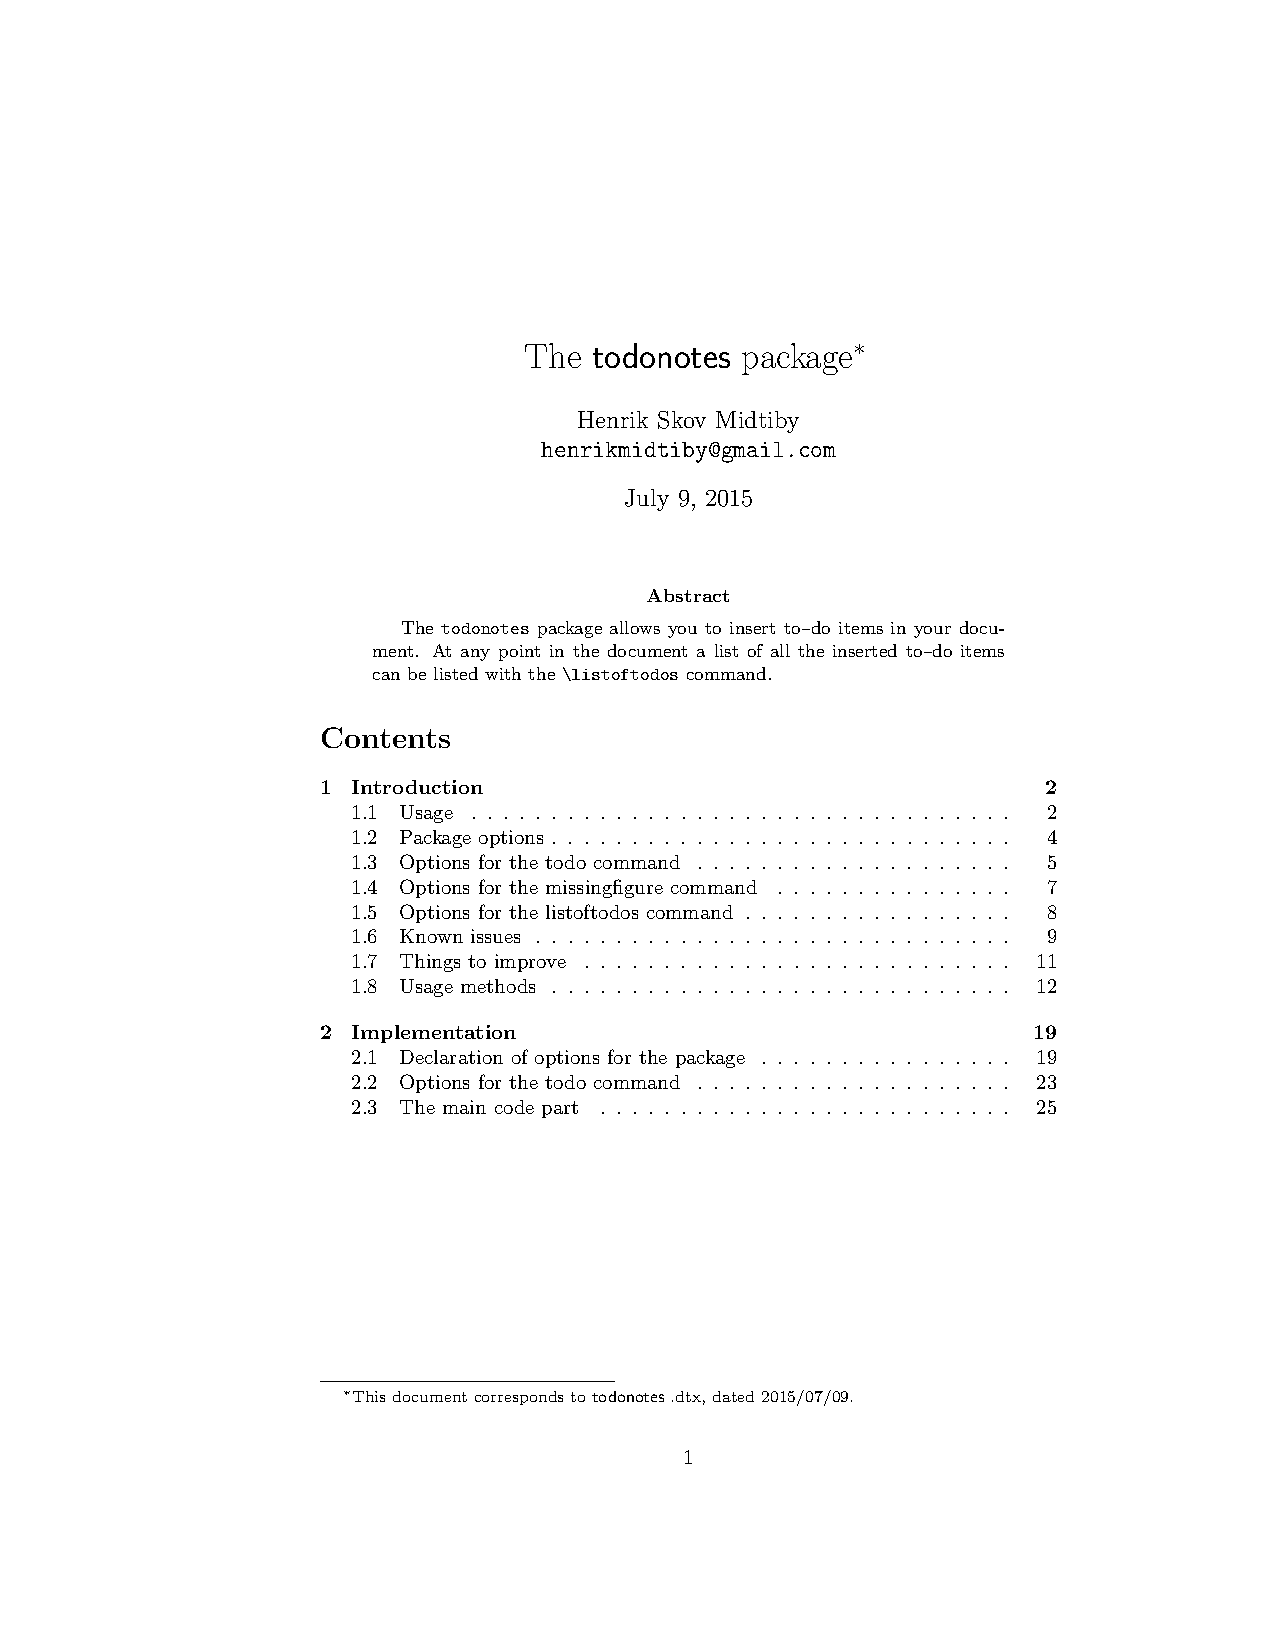
\includepdf[pages=1-3,scale=0.8,frame=true,pagecommand={}]{anexos/todonotes.pdf}
	
	
	% ---
	% Para incluir sem gerar a quebra de página inicial no anexo
	\chapter{Publicações no Blog}
	
	Esse apêndice trás os posts do blog semanal para demonstrar o desenvolvimento do projeto ao decorrer da matéria. 
	
	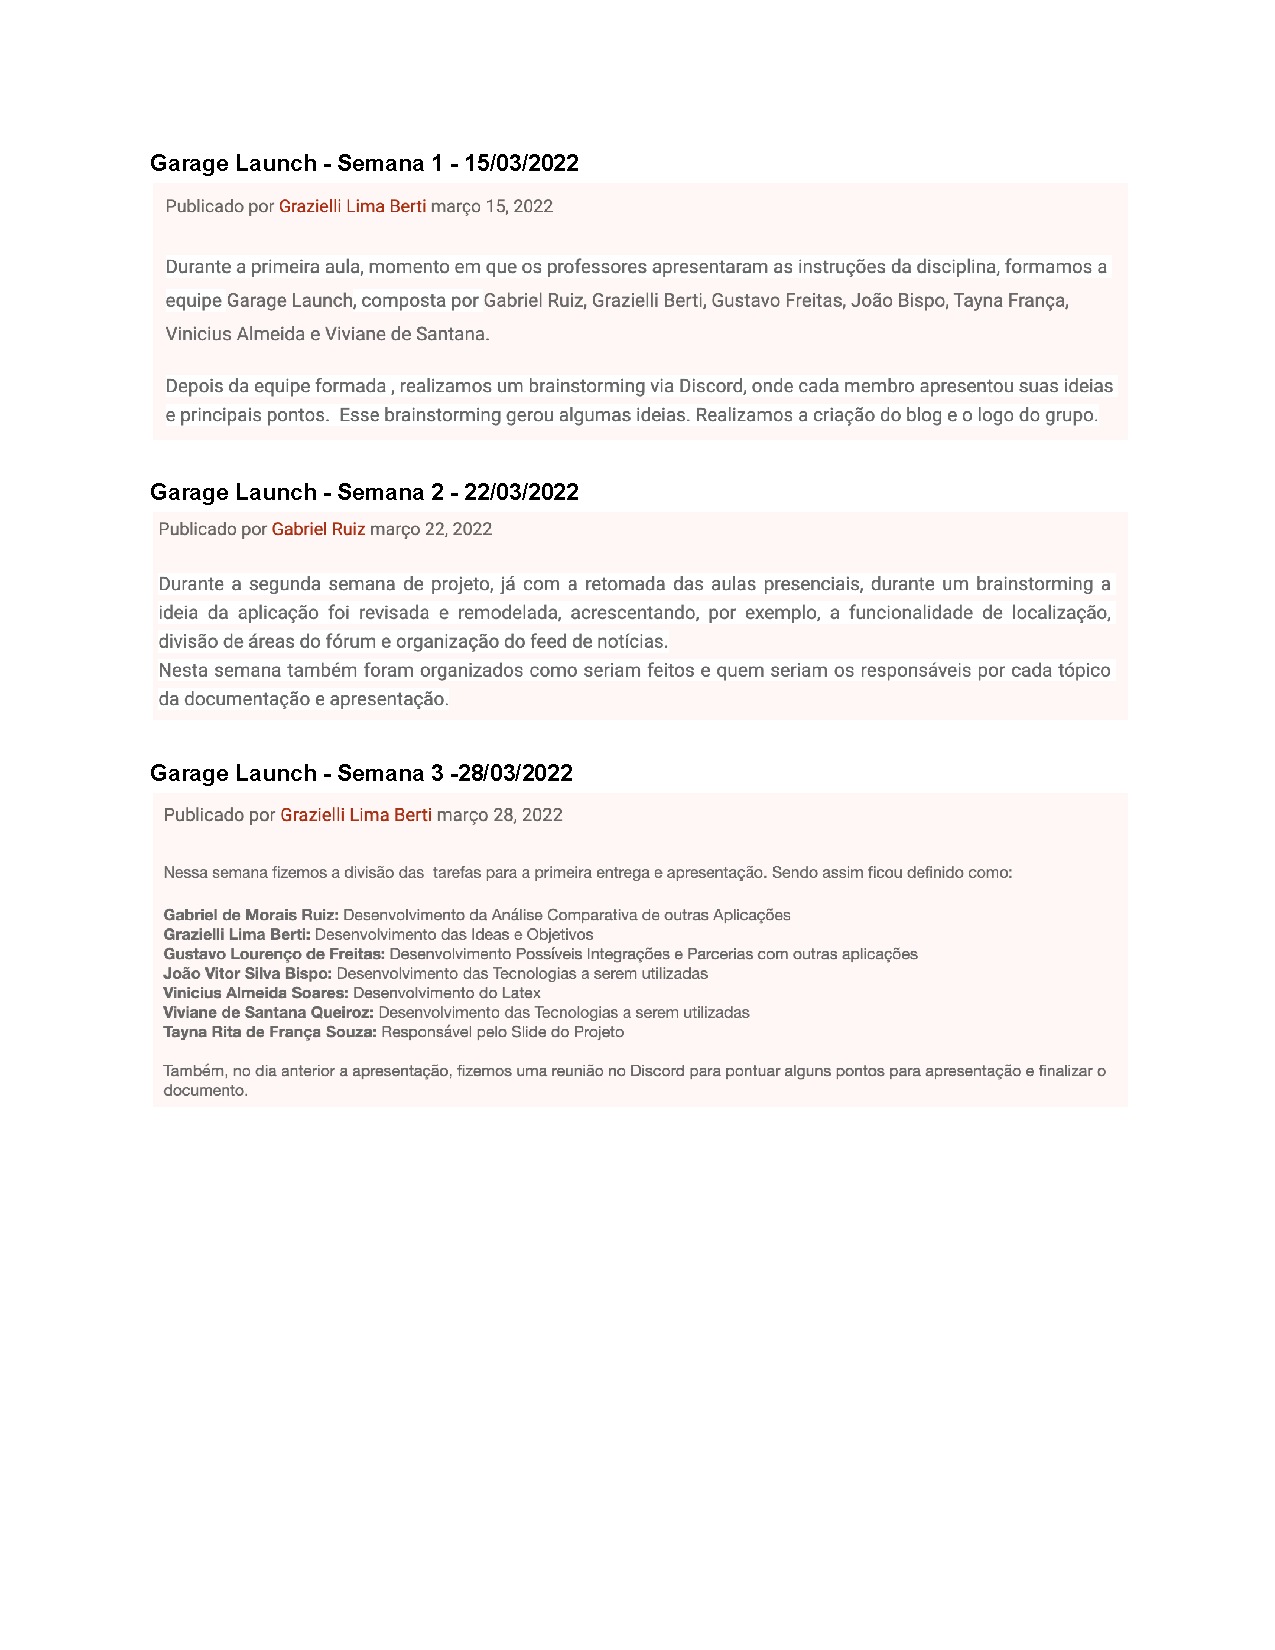
\includepdf[pages=1-6,scale=0.9,frame=true,pagecommand={}\label{publicacao-blog}]{anexos/Anexos_Todos_Os_Post_Do_Blog.pdf}
	
	
\end{apendicesenv}
% ---
